% Title: glps_renderer figure
% Creator: GL2PS 1.3.8, (C) 1999-2012 C. Geuzaine
% For: Octave
% CreationDate: Thu Jun 26 12:41:04 2014
\setlength{\unitlength}{1pt}
\begin{picture}(0,0)
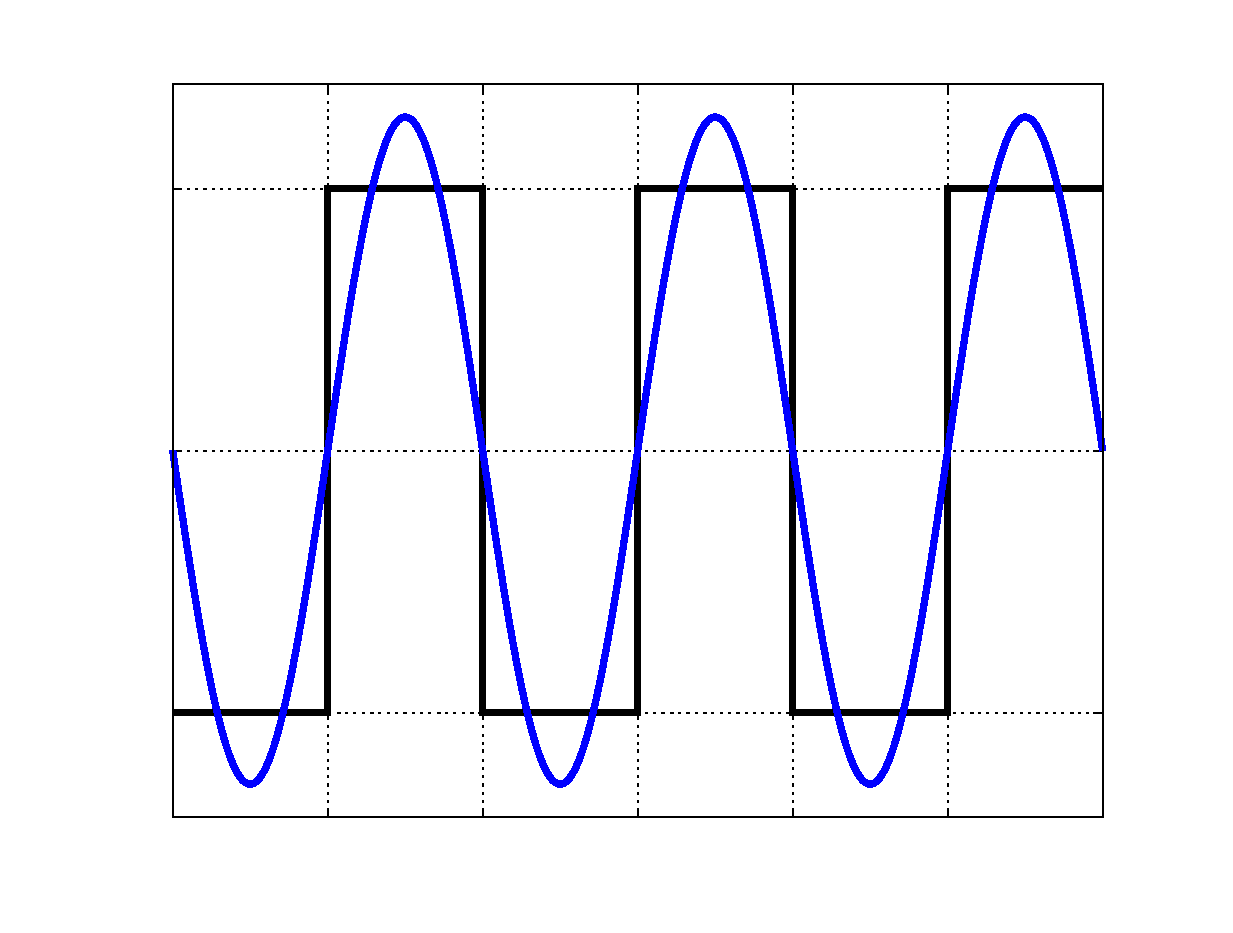
\includegraphics{CuadradaAproximaciones1-inc}
\end{picture}%
\begin{picture}(576,432)(0,0)
\fontsize{30}{0}
\selectfont\put(149.28,42.519){\makebox(0,0)[t]{\textcolor[rgb]{0,0,0}{{-2$\pi$}}}}
\fontsize{30}{0}
\selectfont\put(223.68,34.5){\makebox(0,0)[t]{\textcolor[rgb]{0,0,0}{{-$\pi$}}}}
\fontsize{30}{0}
\selectfont\put(298.08,42.519){\makebox(0,0)[t]{\textcolor[rgb]{0,0,0}{{0}}}}
\fontsize{30}{0}
\selectfont\put(372.48,34.5){\makebox(0,0)[t]{\textcolor[rgb]{0,0,0}{{$\pi$}}}}
\fontsize{30}{0}
\selectfont\put(446.88,42.519){\makebox(0,0)[t]{\textcolor[rgb]{0,0,0}{{2$\pi$}}}}
\fontsize{30}{0}
\selectfont\put(69.8755,97.8169){\makebox(0,0)[r]{\textcolor[rgb]{0,0,0}{{-1}}}}
\fontsize{30}{0}
\selectfont\put(69.8755,223.56){\makebox(0,0)[r]{\textcolor[rgb]{0,0,0}{{0}}}}
\fontsize{30}{0}
\selectfont\put(69.8755,349.303){\makebox(0,0)[r]{\textcolor[rgb]{0,0,0}{{1}}}}
\end{picture}
